
\documentclass[10pt]{article}
\usepackage{fullpage,enumitem,amsmath,amssymb,graphicx}
\usepackage{listings}
\usepackage{amsmath, amssymb}
% \usepackage{stix}
\usepackage{booktabs}
\usepackage{tikz}
\usetikzlibrary{bayesnet}
\usepackage{algorithm}
\usepackage{algorithmic}
\usepackage{hyperref}

\begin{document}
%{{{ header
\begin{center}
{\Large CS 228 Winter 2018 Homework 1}

\begin{tabular}{rl}
SUNet ID: & 05794739 \\
Name: & Anass Belcaid \\
Collaborators: & \\
Late Days: & 2
\end{tabular}
\end{center}

By turning in this assignment, I agree by the Stanford honor code and declare
that all of this is my own work.
%}}}
%{{{ Probability Theory
\section*{Problem 1: Probability theory (4 points)}

The doctor  has bad news and good news for $X$. The bad news is that $X$ tested
positive for a serious disease and the test is $99\%$ accurate. The good news is
that is a rare disease, striking at only one in 10,000 people.

\begin{itemize}
  \item What it is a good news that the disease is rare?
    \item What are the chances that $X$ has actually the disease?
  \end{itemize}

\begin{enumerate}[label=(\alph*)]
  \item The fact that the disease is rare makes the prior $P(D=1)=10^{-5}$ makes
    the probability of having the disease so small even if the test is positive.
    \item Let denote by $D$ the probability of having the disease, hence, we
      have $P(D=1) = 10^{-5}$. Also we will denote the conditional probability
      $P(D | T)$ of having the disease $D$ given the the result of the test $T$.

      Hence the query probability is :

      \begin{eqnarray}
        P(D | T) & = & \dfrac{ P(T | D)\; P(D)}{P(T)}\\
                 & = & \dfrac{P(T|d=1)P(D=1) }{ P(T|D=1)P(D=1) + P(T|D=0)P(D=0)  }\\
                 & = & \dfrac{ 0.99\times 0.00001}{ 0.99\times 0.00001 + 0.01\times0.99999} \\
                 & \approx & 0.98\%
        \end{eqnarray}
\end{enumerate}

Therefore even if the test is $99\%$, the probability of $X$ to have to disease
is still very \textbf{low}.
\section*{Problem 2: Review of dynamic programming (7 points)}
Suppose you have a probability distribution $P$ over the variables $X_1, X_2,
\ldots, X_n$ which all take values on the set $\mathcal{S}=\{v_1, \ldots, v_m\}$ where
$v_j$ are some distinct variables (digits or letters). Suppose that $P$
satisfies the \emph{Markov assumption} for all $i\geq 2$ we have:


\begin{equation}
  \label{eq:markov_assumption}
  P(x_i| x_{i-1}, \ldots, x_1) = P(x_i| x_{i-1})
  \end{equation}
  In other word $P$ factorizes as

 \begin{equation}
   P(x_1,x_2,\ldots, x_n)  = P(x_1)P(x_2|x_1)P(x_2|x_1)\ldots P(x_n|x_{n-1})
   \end{equation}

   for each $i\geq 2$, you are given the factor $P(x_i|x_{i-1})$ as an $m\times
   m $ table and you are given the table $P(x_1= v)$ for each $v \in
   \mathcal{S}$.

\begin{itemize}
  \item Give an $\mathcal{O}(m^2n)$ algorithm for solving the problem
\begin{equation}
  \label{eq:max_prob_markov}
  \max_{x1,\ldots,x_m \in \mathcal{S}^n} P(x_1) P(x_2|x_1)\ldots P(x_n|x_{n-1})
  \end{equation}
  \end{itemize}
\begin{enumerate}[label=(\alph*)]
  \item In order to solve the problem in Eq.\ref{eq:max_prob_markov}, we propose
    the following \emph{reduction} to the problem
   
\begin{equation}
  \max_{x1,\ldots,x_m \in \mathcal{S}^n} P(x_1,\ldots,x_n) = \max_{x_n, x_{n-1}} P(x_n|x_{n-1})\max_{x_1,\ldots,x_{n-1}} P(x_1)\ldots P(x_{n-1}| x_{n-2})
  \end{equation}

\begin{itemize}
  \item The first maximization could be solved in quadratic time
    $\mathcal{O}(m^2)$, since we need to check all the possible values for $x_n$
    and $x_{n-1}$.
   \item By doing so, we simplified the problem from computing the
     \textbf{maximum} over $n$ variable to a maximum of $n-1$ variables. hence,
     we will repeat the simplification until we obtain the unique factor $P(x_1)$.
\end{itemize}
\end{enumerate}
\begin{algorithm}[H]
  \begin{algorithmic}
    \REQUIRE factors $P(x_i|x_{i-1})$

    \STATE initialize $\mathbf{M}\in \mathbf{R}^m$ with $P(x_1= v\in\mathcal{S})$


    \FOR{ i = 1 \TO n}
    \FOR { j = 1 \TO m}
    \STATE $\text{max\_value } = -\infty$
    \FOR{k = 1 \TO m}
    \STATE $\text{max\_value} = \max(\text{max\_value}, M[j]\times P(X_i=v_k|V_{i-1}=v_j))$
    \ENDFOR
    % \STATE $M[i] = \text{max\_value}$
    \ENDFOR

    \ENDFOR
    
    \end{algorithmic}
  \caption{Dynamic programming to solve the maximization problem}
  \end{algorithm}
  %}}}
%{{{ Problem 3: Bayesian network
\section{Problem 3: Bayesian Network (6 points)}
Let's try to relax the definition of \emph{Bayesian network} by removing the
assumption that the directed graph is acyclic. Suppose that we have a directed
graph $G = (V,E)$ and a discrete random variables $X_1,\ldots, X_n$ and define:

\begin{equation}
  \label{eq:decomposition_bayesian}
  f(x_1,\ldots,x_n) = \prod_{v \in V} f_v(x_v| x_{pa}(v))
\end{equation}
where $x_{pa}$ refers to the parents of of the variable $X_v$ in $G$ and $f_v$
specifies the distribution over the $X_v$ for every assignment of the parents.
We recall that Eq.\ref{eq:decomposition_bayesian} is  precisely the definition
of the joint probability associated with Bayesian network $G$, where $f_v$ are
the conditional probabilities.

\begin{itemize}
  \item Show that if the graph has a directed cycle, $f$ do no longer define a
    probability distribution.
    \item In particular, give an example of a cyclic graph $G$ and a
      distribution $f_v$ that lead to improper probabilities.
  \end{itemize}


\begin{enumerate}[label=(\alph*)]
\item Let's consider the simple bayesian network

  \begin{center}
    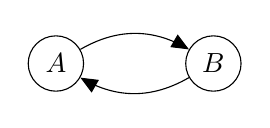
\begin{tikzpicture}
\node[latent] (A) at (0,0) {$A$};
\node[latent] (B) at (2,0) {$B$};
\path[draw,->] (A)edge [bend left](B);
\path[draw,->] (B)edge [bend left](A);
      \end{tikzpicture}
  \end{center}

with the following tables $P(A|B) = \begin{bmatrix} & b_0 & b_1\\ a_0 & 1 & 0\\
  a_1 & 0 & 1  \end{bmatrix}$ and $P(B|A) = \begin{bmatrix} & a_0 & a_1\\ b_0 & 0.7 & 0.5\\
  b_1 & 0.3 & 0.5  \end{bmatrix}$.

With this choice we get
$$
\begin{array}{ll}
  \toprule
  a,b & P(a,b) \\
  \midrule
  (a_0,b_0) &  0.7\\
  (a_0,b_1) &   0 \\
  (a_1,b_0) &   0 \\
  (a_1,b_1) &   0.5\\
  \bottomrule
  \end{array}
$$

we clearly is not a probability distribution since $\sum_{a,b} P(A,B) \neq 1$.
  \end{enumerate}
%}}}
%{{{ Conditional Independence
\section{Problem 4: Conditional Independence (12 points)}

The question investigates the way  in which  conditional independence
relationship affect the amount of information needed for probabilistic
graphical calculations. Let $\alpha$ and $\beta$ and $\gamma$ be three random
variables.


\begin{itemize}
  \item (6 points)  Suppose we wish to calculate $P(\alpha| \beta, \gamma)$ and
    we have no conditional independence information. Which of the following set
    of number is sufficient for the calculations?
   \begin{enumerate} 
     \item $P(\beta, \gamma)$, $P(\alpha)$, $P(\beta|\alpha)$ and $P(\gamma|\alpha)$.
       \item $P(\beta,\gamma)$, $P(\alpha)$ and $P(\beta, \gamma|\alpha)$
         \item $P(\beta|\gamma)$, $P(\gamma|\alpha)$ and $P(\alpha)$
     \end{enumerate}
     for each case either give the method to calculate the probability or why
     it's not sufficient to compute the posterior.

     \item (6 points) Suppose we know $\beta$ and $\gamma$ are independent given
       $\alpha$. Now which one of preceding probabilities is sufficient.
  \end{itemize}
  
\begin{enumerate}[label=(\alph*)]
\item For the first case the probability $P(\gamma,\beta)$ is the probability of
  the conditioned event. Hence, we need to express the probability
  $P(\alpha,\beta,\gamma)$ with the remaining expressions. we have $P(\alpha)$
  and $P(\beta|\alpha)$ the third one need to \textbf{forcefully } to be
  conditioned on $\alpha$ and $\beta$.\\

  \item The second one could be used to get the posterior using \emph{Bayes}
    rule

    \begin{equation}
      P(\alpha| \beta, \gamma) = \dfrac{P(\alpha) P(\beta,\gamma|\alpha)}{P(\beta,\gamma)}
      \end{equation}

    \item For the third one, we can no longer calculate the probability of the
      conditioned event $P(\beta, \gamma)$ by the given expressions.
  \end{enumerate}
  
\begin{enumerate}[label=(\alph*)]
  \item If we have the information $\beta $ and $\gamma$ are independent given
    $\alpha$ we could use the entities in the \textbf{first} proposition by

    \begin{equation}
     P(\alpha|\beta,\gamma)  = \dfrac{P(\alpha)P(\gamma|\alpha)P(\beta|\alpha)}{P(\gamma, \beta)}
      \end{equation}
  \end{enumerate}
  %}}}
%{{{ Bayesian Network
\section{Bayesian network (AD exercice 4.1): (5 points)}

\begin{enumerate}[label=(\alph*)]
\item From the graph, the nodes $A$ and $B$ are independents.

  $$
  P(A=0, B = 0) = P(A=0)P(B=0) = 0.8 \times 0.3 = 0.24
  $$

  for the second P(E=1|A = 1), since there is no active \textbf{trail} from $A$
  to $E$ the two variables are independents. Hence $P(E=1|A=1) = P(E=1)$.


  $$
  P(E=1) = \sum_B P(E=1|B)P(B) = 0.7\times0.1 + 0.3\times0.9 = 0.34
  $$

 \item Are $A$ and $E$ D-separable given $E$ and $H$. No since there is an
   active trail $A-C-F-H-E$ leading from A to E. The trail is active since it
   contains the $V-$ structure $F-H-E$.
  \item Are $G$ and $E$ D-separable given $D$. Yes since there is no active path
    from $G$ to $E$ or vise-versa
    \item  Are ${A,B}$ and ${G,H}$ D-separable given $F$. \textbf{False} since
      there is a clear path $B-E-H$.
\end{enumerate}
%}}}
%{{{ Bayesian Network expaling away
\section{Bayesian networks: Explaining away (7 points)}

You want to model the admission process of Farm university. Students are
admitted based on their Creativity (C) and Intelligence (I). You decide  to
model them as continuous random variables, and your data suggests that both are
uniformly distributed in $[0,1]$, and are independent of each other. Formally
$I\sim\mathcal{U}([0,1])$, $C\sim\mathcal{U}([0,1])$ and $I \perp C$.

Being very prestigious the school only admits student such as $I + C \geq 1.5$

\begin{enumerate}
\item (1 points) What is the expected creativity score of a student?
  \item (2 points) What is the expected creativity score of an admitted student?
    \item (2 points) What is the expected creativity  score of a student with $I=0.95$.
    \item (2 points) What is the expected creativity score of an admitted
      student with intelligence $I=0.95$? How does this score compares to the
      question 3?
\end{enumerate}

\begin{enumerate}[label=(\alph*)]
\item Let's draw the graphical model for the three variables

  \begin{center}
    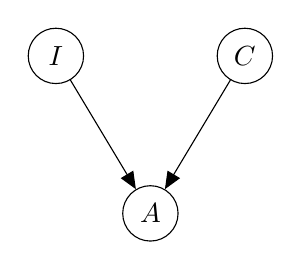
\begin{tikzpicture}[xscale=0.6]
      \node[latent] at (0,0) (I) {$I$};
      \node[latent] at (4,0) (C) {$C$};
      \node[latent] at (2,-2) (A) {$A$};
      \edge[->]{I}{A}
      \edge[->]{C}{A}
      \end{tikzpicture}
    \end{center}
Since the single variable $I\sim \mathcal{U}(0,1)$, its expectation $E(I) = 0.5$.
\item The expected creativity of an admitted student is :

 \begin{equation}
   E(C | A = 1) = \int_0^1 c P(c|A=1)dc
   \end{equation}
Or We need to compute the probability of the event $A$.

\begin{eqnarray}
  P(A) &=& \int_c \int_i f_I\;f_C di\;dc\\
       &=& \int_{.5}^1 di\int_{1.5-i}^1dc\\
       &=&=\dfrac{1}{8} \\
\end{eqnarray}

and the conditioned probability probability density $f_{c|A}$ is given by:

\begin{equation}
  f_{c|A}=\left\{\begin{array}{ll}
      \dfrac{1}{8} & \text{if } A\\[8pt]
      0            & \text{otherwise}
  \end{array}\right.
\end{equation}

Finally the expected creativity $E(c|A)$ is given by:

\begin{equation}
  E(C|A) = \int_{.5}^1di\int_{1.5-i}^1 cdc = \dfrac{5}{6}
\end{equation}

\item Given the graphical model, the variable $\mathbf{C}$ is independent of the
  intelligence.
  Therefore:

  \begin{equation}
    E(C|I=0.95) = E(C) = 0.5
  \end{equation}

\item In order to compute the  expected creativity of an admitted student with
  Intelligence $I=0.95$, We need to compute the probability of the event $A$
  and $I=0.85$.

  \begin{equation}
    P(A, I=0.95) = \int_{c=0.55}^1 dc = 0.45
  \end{equation}


Given that, the conditioned expectation $E(C|A, I=0.95)$ is given by:

\begin{equation}
  E(C|A, I=0.95) = \int_{.55}^1 \dfrac{c}{0.45}dc=\mathbf{0.77}
\end{equation}
The expected creativity did decrease indicating the dependence of the two
variables $I$ and $C$ given we observed the common effect $A$.
\end{enumerate}
%}}}
%{{{Problem  8 Bayesian Networks
\section{Bayesian Networks (3.11 from Kroller)}%
\label{sec:bayesian_networks}
\begin{figure}[ht!]
\begin{center}
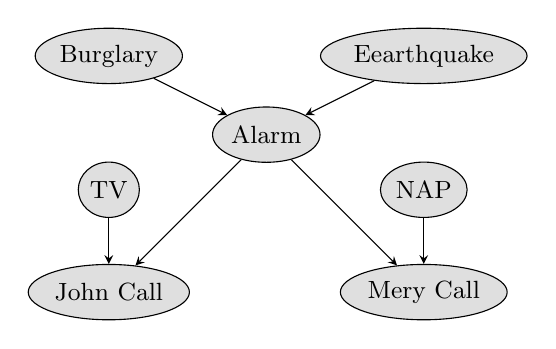
\begin{tikzpicture}[scale=1,>=stealth]
  \node[obs,ellipse]  at (0,0) (bulg) {\small Burglary};
  \node[obs,ellipse]  at (4,0) (earth) {\small Eearthquake};
  \node[obs,ellipse]  at (2,-1) (alarm) {\small Alarm};
  \node[obs,ellipse]  at (0,-1.7) (tv) {\small TV};
  \node[obs,ellipse]  at (4,-1.7) (nap) {\small NAP};
  \node[obs,ellipse]  at (0,-3) (john) {\small John Call};
  \node[obs,ellipse]  at (4,-3) (Mery) {\small Mery Call};
  \edge{bulg}{alarm}
  \edge{earth}{alarm}
  \edge{alarm}{john,Mery}
  \edge{tv}{john}
  \edge{nap}{Mery}
\end{tikzpicture}
\end{center}
\caption{Bayesian network from Kroller 3.11}%
\label{fig:bayesian_network}
\end{figure}

\begin{enumerate}
  \item (8 points) Consider the Burglary alarm given in
    figure~\ref{fig:bayesian_network}. Construct a Bayesian Network  over all
    the node \textbf{except} the \emph{Alarm} That is a minimal \emph{I-map} for
    the marginal distribution over the remaining variables.\footnote{Be sure to
    get all the dependencies from the original graph}.

    Let's redraw the network by taking the first letter of each variable ans
    making the variable \texttt{Alarm} oberved.

\begin{center}
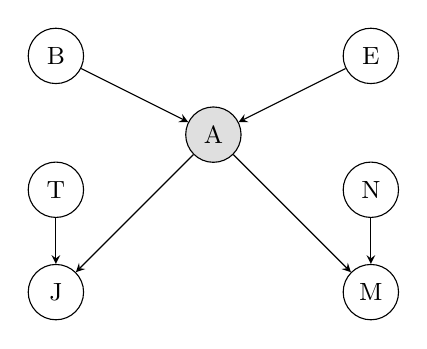
\begin{tikzpicture}[scale=1,>=stealth]
  \node[latent,ellipse]  at (0,0) (bulg) {\small B};
  \node[latent,ellipse]  at (4,0) (earth) {\small E};
  \node[obs,ellipse]  at (2,-1) (alarm) {\small A};
  \node[latent,ellipse]  at (0,-1.7) (tv) {\small T};
  \node[latent,ellipse]  at (4,-1.7) (nap) {\small N};
  \node[latent,ellipse]  at (0,-3) (john) {\small J};
  \node[latent,ellipse]  at (4,-3) (Mery) {\small M};
  \edge{bulg}{alarm}
  \edge{earth}{alarm}
  \edge{alarm}{john,Mery}
  \edge{tv}{john}
  \edge{nap}{Mery}
\end{tikzpicture}
\end{center}


We construct a \textbf{topological sorring} of the graph and then for each node
$X_i$, we chooose the minimal set $U$ that eclipse the $X_i$ for the rest of the
other variables $\big(X_i | \{X_0,\ldots, X_{i-1}\} - U | U\big)$.

\begin{center}
  
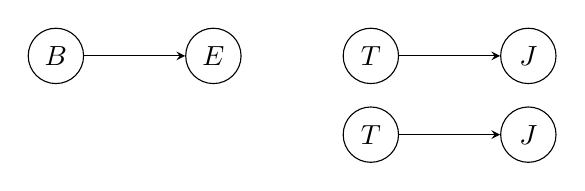
\begin{tikzpicture}[scale=1,>=stealth]
  \node[latent] (B) at (0,0){$B$};
  \node[latent] (E) at (2,0){$E$};
  \node[latent] (T) at (4,0){$T$};
  \node[latent] (J) at (6,0){$J$};
  \node[latent] (N) at (4,-1){$T$};
  \node[latent] (M) at (6,-1){$J$};
  \edge{B}{E}
  \edge{T}{J}
  \edge{N}{M}
\end{tikzpicture}

\end{center}

  \item (8 points) Generalize this procedure to an arbitrary network. More
    precisely, assume we are given a network BN, an ordering $X_1,\ldots,X_n$
    that is consistent with the ordering of the variables in BN and a node $X_i$
    to be removed. Specify a network BN1 is minimal \emph{I-map} for the
    remaining variables.
    Similar to the procedure in \textbf{Koller 3.4(p 79)}, we will start with
    the vraiables $X_1$ eand for each variable $X_i$, we will choose the
    minitmal set $\mathcal{D}$ such as

    \begin{equation}
    X_i\;\perp\i\{X_1,\ldots,X_{i-1}\}-\mathcal{D}\;| \mathcal{D},X_r\}
    \end{equation}

    Once we computed $\mathcal{D}$, we chose the set of its nodes as the parents
    of $X_i$. Therefore, we add an arc $X_j\rightarrow X_i$ for each
    $X_j\in\mathcal{D}$.
\end{enumerate}
%}}}
%{{{Toward inference In Bayesian network
\section{Problem 9 Toward bayesian inference}%
\label{sec:problem_9_toward_bayesian_inference}
\begin{enumerate}
  \item (4 points) Suppose you have  a Bayes net over $n$ nodes
    $\big(X_1,\ldots,X_n\big)$ and all the variables except $X_i$ are
    \textbf{observed}. Using the chain rule and Bayes rule find an efficient
    algorithm to compute the probability:
    \begin{equation}
      P(x_i|x_1,\ldots, x_n)
    \end{equation}
    Lets parition the nodes of the bayesian network according to their relation
    to $X_i$.

\begin{equation}
  \left\{\begin{array}{ll}
      \text{Pa}_i  & \text{parent of } x_i \\
      \text{Ch}_i & \text{childs of } x_i\\
      \text{O}_i & \text{others}\\
  \end{array}\right.
\end{equation}

Using the Bayes rule we obtain:

\begin{equation}
P(x_i|x_1,\ldots, x_n) = \dfrac{P\big(x_i|x_1\ldots,x_n\big)}{\sum_{x_i} P\big(x_i|x_1\ldots
x_n\big)}
\end{equation}

Using the nodes decomposition, we obtain

\begin{equation}
P(x_i|x_1,\ldots,x_n) = \dfrac{P(x_|Pa(x_i) \prod_{x\in Ch_i} P(x|Pa(x)\big)}
{\sum_{x_i} P(x_i|Pa(x_i) \prod_{x \in Ch_i}P(x|Pa(x)}
\end{equation}

\begin{center}
  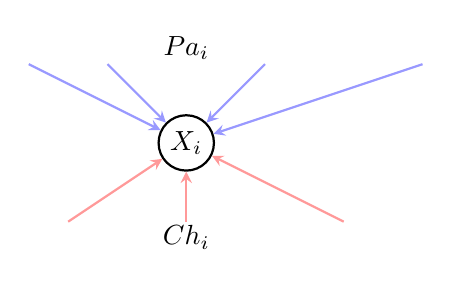
\begin{tikzpicture}
    \node[latent, ellipse,thick] (xi) at (0,0) {$X_i$};
    \foreach \x in {-2,-1, 1, 3}
    \draw[thick,->,color=blue!40,>=stealth] (\x, 1) -- (xi);
    \node at (0,1.2) {$Pa_i$};

    \foreach \x in {-1.5,0, 2}
    \draw[thick,->,color=red!40,>=stealth] (\x, -1) -- (xi);
    \node at (0,-1.2) {$Ch_i$};
  \end{tikzpicture}
\end{center}
The entities should be computed for each values $x_i$ in order to evaluate the
partition normalizing factor.

\item (4 points) Find an efficient algorithm to generate random samples from the
  probability distribution defined in a Bayesian Network. You can assume access
  to a routine to draw a sample from \emph{multinomial}.
  Let's consider the simple case $X\rightarrow Y$. By using the chain rule,
  $P(x,y) = P(x) P(y|x)$, we could draw a sample by using the procedure from a
  multinomial $\mathcal{M}$ as:

  $$
  x = \mathcal{M}(X)\quad, \quad y=\mathcal{M}(Y|x)
  $$

  Hence for any \emph{BN} defined by the decomposition $P(x1,\ldots,x_n)=\prod
  P\big(x_i|Pa(x_i)\big)$, we start from the root\footnote{A DAG accepts a
  topological ordering} and for each $x_i$ we draw a sample using 
  \begin{equation}
    \mathcal{M}(x_i| Pa(x_i) = \text{sample})
  \end{equation}
\end{enumerate}

%}}} end Toward inference In Bayesian network
%{{{Programming Assignment
\section{Programming Assignment}%
\label{sec:programming_assignment}

\begin{enumerate}
  %{{{ number of possible images
  \item  Since each pixel could take a values on $\{0,1\}$, the set of binary
    images of size $28\times 28$ is $\vert I_{28,28}\vert =\mathbf{2}^{784}$
    %}}}
    %{{{ Number parameters full
  \item The number of parameter without conditioning is $2^{784} - 1$. 
    %}}}
    %{{{ Number of parameter
  \item  For the Bayesian Net the probability distribution is written as:

    \begin{equation}
      P(X_1,\ldots, X_{784}, Z_1, Z_2) =  P(Z_1)P(Z_2) \prod_i P(X_i|Z_1, Z_2)
    \end{equation}
    We need $\mathbf{784}$ conditional $P(X_i|Z_1, Z_2)$ probability for each
    $X_i$. The cardinality of a latent variable is $25$. Therefore for each
    CPD, we need $25\times 25 -1 = \mathbf{624}$ parameter.\\

    Therefore, the number of parameters is $784\times 624 = 489216$.
    %}}}
    %{{{ Question 4 on generating samples
  \item  Here is the result, in \autoref{fig:q4},  of the sampling from the model:

    \begin{figure}[htpb]
      \centering
      \includegraphics[width=0.8\linewidth]{./programming/a4.png}
      \caption{Sampling the Learned distribution}%
      \label{fig:q4}
    \end{figure}
    %}}}
%{{{Excpected images
  \item The expected images are depicted on \autoref{fig:expected_images}.

%{{{
    \begin{figure}[htpb]
      \centering
      \includegraphics[width=0.8\linewidth, height=6cm]{./programming/a5.png}
      \caption{Excpected image for each latent value}%
      \label{fig:expected_images}
    \end{figure}
    %}}}
  \item We will classify the images according to the log-likehood

    \begin{equation}
      \label{eq:log_likelihood}
   P(X_{1:784}) = \log \sum_{z_1}\sum_{z_2} p(z_1,z_2) \prod_i p(X_i|z_1,z_2)
    \end{equation}


 The proposed classifier will compute the mean and the standard deviation on the
 \emph{validation} Dataset. For each image on the \emph{Test}, An image is
 classified as normal is the lies within three standard deviation from the
 validation mean.

 \begin{figure}[ht]
   \centering
   \includegraphics[width=0.8\textwidth, height=6cm]{./programming/positive.png}
   \caption{Histogram of the positive images}
 \end{figure}


 \begin{figure}[ht]
   \centering
   \includegraphics[width=0.8\textwidth, height=6cm]{./programming/negative.png}
   \caption{Histogram of the negative images}
 \end{figure}

\item Question 7: visualize the scatter plot for the expected latent variables

  \begin{figure}[ht]
    \centering
    \includegraphics[width=15cm, height=8cm]{./programming/q7.png}
    \caption{Distribution of the latent variables expectations }
  \end{figure}

    % }}} end Excpected images
\end{enumerate}
%}}} end Programming Assignment
\end{document}




